\chapter{Architektura i wdrożenie środowiska laboratoryjnego}\label{ch:architektura_laboratorium}

\section{Założenia architektoniczne i izolacja sieciowa}\label{sec:izolacja_sieciowa}

Fundamentem eksperymentu jest utworzenie odizolowanego, powtarzalnego środowiska wirtualnego, które uniemożliwia wyciek szkodliwego kodu poza kontur badawczy, a jednocześnie dostarcza analizowanym próbkom wiarygodne syntetyczne odpowiedzi sieciowe. Schemat topologii oraz podział ról w sieci przedstawiono na rysunku~\ref{fig:topologia_lab}.

\begin{figure}[htbp]
    \centering
    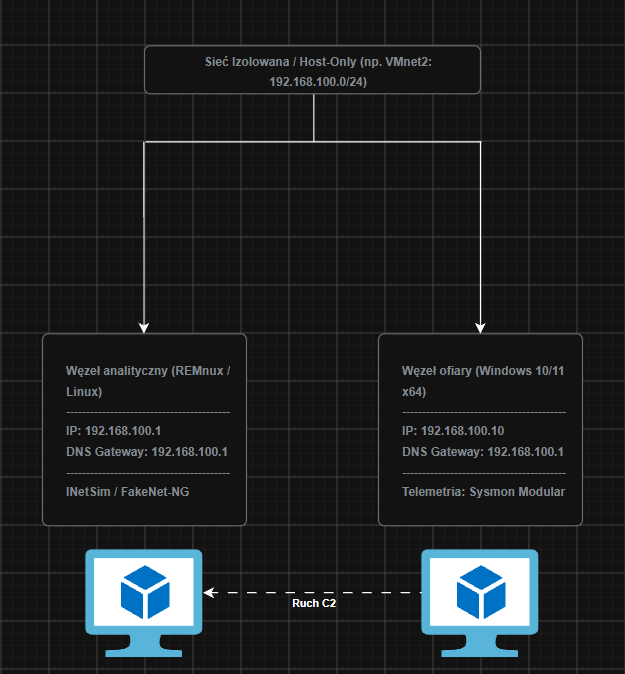
\includegraphics[width=0.85\linewidth]{images/topology.png}
    \caption{Topologia połączeń i podział ról w odizolowanej podsieci laboratoryjnej}
    \label{fig:topologia_lab}
\end{figure}

Do realizacji projektu wykorzystano hiperwizor typu 2 (\textit{Type-2 Hypervisor}) VMware Workstation Pro. Wybór tego środowiska wynika z natywnego wsparcia dla formatu pamięci migawek (\file{.vmem}), który jest bezpośrednio odczytywany przez frameworki \textit{Volatility 3} oraz \textit{MemProcFS} bez konieczności uruchamiania dodatkowych agentów wewnątrz infekowanej maszyny.

Współpraca węzłów odbywa się w ramach dedykowanej sieci wirtualnej typu \textit{Host-Only} (\code{VMnet2}) z wyłączonym serwerem DHCP hiperwizora oraz całkowicie zablokowanym routingiem do fizycznej karty sieciowej hosta. Adresacja IP została skonfigurowana statycznie i ujęta w tabeli~\ref{tab:adresacja_sieciowa}.

\begin{table}[htbp]
\centering
\caption{Konfiguracja adresacji wirtualnej podsieci badawczej}
\label{tab:adresacja_sieciowa}
\begin{tabularx}{\linewidth}{l l L{3.5cm} Y}
\toprule
\hcell{Węzeł} & \hcell{Adres IP} & \hcell{Rola w sieci} & \hcell{Opis interfejsu} \\
\midrule
REMnux & \code{192.168.100.1} & Brama domyślna / DNS & Pętla symulacji C2 (INetSim / FakeNet-NG) \\
Windows Victim & \code{192.168.100.10} & Stacja ofiary & Punkt detonacji próbek złośliwego oprogramowania \\
\bottomrule
\end{tabularx}
\end{table}

\section{Przygotowanie stacji ofiary i konfiguracja telemetrii}\label{sec:konfiguracja_windows}

Maszyna ofiary bazuje na 64-bitowym systemie Microsoft Windows XXX. Celem zapewnienia niezakłóconego wykonania próbek złośliwego oprogramowania oraz pełnej rejestracji artefaktów podjęto następujące kroki konfiguracyjne:

\subsection{Dezaktywacja mechanizmów obronnych}
Aplikacje typu \textit{Infostealer} oraz \textit{RAT} często przerywają działanie w przypadku wykrycia aktywnych mechanizmów ochronnych. Aby zagwarantować pełne wykonanie ładunku (stadium \textit{post-exploitation}), wyłączono następujące moduły:
\begin{enumerate}
\item \textbf{Windows Defender \& SmartScreen:} Trwale zdezaktywowane za pomocą dedykowanych polis GPO oraz rejestru systemowego:
POPRAWIC
\item \textbf{Antimalware Scan Interface (AMSI):} Ominięte na poziomie pamięci procesu w celu uniemożliwienia skanowania skryptów PowerShell/VBScript.
\item \textbf{Windows Update:} Zablokowane powiązane usługi systemowe, unikając niekontrolowanych zmian w strukturach jądra i wersjach bibliotek DLL.
\end{enumerate}

\subsection{Wdrożenie i dostrojenie rozszerzonej telemetrii (Sysmon)}
Standardowe dzienniki Windows Event Log nie dostarczają dostatecznej szczegółowości w obszarze tworzenia zdalnych wątków czy dostępu do pamięci procesów. Na stacji wdrożono narzędzie \textbf{Microsoft Sysmon} z profilowaniem \textit{Sysmon-Modular}.

Zainstalowano usługę komendą:
\begin{verbatim}
Sysmon64.exe -i sysmonconfig-export.xml
\end{verbatim}

Kluczowe identyfikatory zdarzeń (Event ID) skonfigurowane w profilu pod kątem analizy poinfekcyjnej ujęto w tabeli~\ref{tab:sysmon_events}.

\begin{table}[htbp]
\centering
\caption{Konfiguracja reguł audytu Sysmon na stacji badawczej}
\label{tab:sysmon_events}
\begin{tabularx}{\linewidth}{c L{4.5cm} Y}
\toprule
\hcell{Event ID} & \hcell{Nazwa Zdarzenia} & \hcell{Cel analityczny / Wykrywane techniki} \\
\midrule
1 & Process Creation & Śledzenie drzewa procesów, parametrów CLI, wywołań LOLBins. \\
6 & Driver Loaded & Wykrywanie ładowania nielicencjonowanych sterowników (rootkity / BYOVD). \\
7 & Image Loaded & Rejestracja ładowanych bibliotek DLL (wsparcie detekcji iniekcji). \\
8 & CreateRemoteThread & Kluczowe dla detekcji \textit{Process Injection} oraz \textit{Process Hollowing}. \\
10 & ProcessAccess & Wykrywanie odczytu pamięci \file{lsass.exe} (kradzież poświadczeń). \\
11 & FileCreate & Rejestracja zrzucanych ładunków executable oraz plików persystencji. \\
13 & RegistryEvent & Monitorowanie kluczy autostartu (\code{Run}, \code{RunOnce}, \code{Services}). \\
\bottomrule
\end{tabularx}
\end{table}

\subsection{Optymalizacja buforów EVTX}
Standardowy rozmiar pliku dziennika \file{Microsoft-Windows-Sysmon/Operational.evtx} (20 MB) jest niewystarczający podczas intensywnej infekcji i prowadzi do nadpisywania zdarzeń. Zwiększono limity buforów do 256~MB komendą \code{wevtutil}:
\begin{verbatim}
wevtutil sl "Microsoft-Windows-Sysmon/Operational" /ms:268435456
wevtutil sl "Security" /ms:268435456
\end{verbatim}

\section{Konfiguracja węzła analityczno-symulacyjnego (REMnux)}\label{sec:konfiguracja_remnux}

Węzeł analityczny oparto na dystrybucji REMnux (Linux bazujący na Ubuntu), będącej zestawem gotowych narzędzi inżynierii wstecznej i śledczej.

\subsection{Symulacja usług sieciowych (INetSim / FakeNet-NG)}
Większość współczesnych próbek złośliwego oprogramowania przed przejściem do właściwej fazy ataku sprawdza dostępność łączności z siecią Internet poprzez zapytania DNS lub pobranie testowego pliku HTTP. Brak odpowiedzi powoduje przedwczesne zakończenie procesu.

Na stacji REMnux skonfigurowano pakiet \textbf{INetSim}, który nasłuchuje na interfejsie \code{192.168.100.1} i udaje powszechne usługi sieciowe:
\begin{itemize}
\item \textbf{DNS Server:} Odpowiada własnym adresem IP (\code{192.168.100.1}) na wszystkie zapytania o nazwy domenowe (np. zapytania C2).
\item \textbf{HTTP/HTTPS Server:} Zwraca poprawne nagłówki statusu \code{200 OK} oraz serwuje syntetyczne pliki binarne w odpowiedzi na żądania pobrania ładunków drugiego stopnia.
\item \textbf{SMTP / IRC / Dummy TCP:} Przechwytuje próby eksfiltracji danych zebranych przez Infostealery.
\end{itemize}

Ruch sieciowy jest równolegle rejestrowany do plików PCAP za pomocą narzędzia \code{tshark}:
\begin{verbatim}
tshark -i eth0 -w /analiza/dumps/capture_infekcja.pcap
\end{verbatim}

\subsection{Stos narzędziowy węzła analitycznego}
Na maszynie REMnux przygotowano kompletny zestaw oprogramowania analitycznego podzielony na trzy środowiska:
\begin{enumerate}
\item \textbf{Analiza pamięci RAM:} Volatility 3 (z pobranymi symbolami PDB dla Windows) oraz MemProcFS.
\item \textbf{Triage i korelacja dzienników:} Chainsaw oraz Hayabusa wyposażone w aktualne reguły Sigma (SigmaHQ).
\item \textbf{Walidacja i inżynieria reguł:} Silnik YARA 4.x oraz narządzia \code{sigma-cli}.
\end{enumerate}

\section{Procedura powtarzalności eksperymentu i akwizycji artefaktów}\label{sec:procedura_akwizycji}

W celu zachowania rygoru badawczego i powtarzalności wyników, dla każdej analizowanej próbki złośliwego oprogramowania stosowana jest ściśle zdefiniowana procedura postępowania przedstawiona na rysunku~\ref{fig:cykl_badawczy}.

\begin{figure}[htbp]
\centering
\begin{verbatim}
┌─────────────────────────────────────────────────────────┐
│ 1. Przywrócenie czystego stanu (Snapshot: Clean_State)  │
└────────────────────────────┬────────────────────────────┘
                             │
                             ▼
┌─────────────────────────────────────────────────────────┐
│ 2. Uruchomienie nasłuchu sieciowego na REMnux (tshark)  │
└────────────────────────────┬────────────────────────────┘
                             │
                             ▼
┌─────────────────────────────────────────────────────────┐
│ 3. Detonacja próbki złośliwego kodu na Windows Victim   │
└────────────────────────────┬────────────────────────────┘
                             │
                             ▼
┌─────────────────────────────────────────────────────────┐
│ 4. Obserwacja poinfekcyjna i aktywność C2 (5-10 min)    │
└────────────────────────────┬────────────────────────────┘
                             │
                             ▼
┌─────────────────────────────────────────────────────────┐
│ 5. Akwizycja RAM (.vmem) oraz eksport dzienników EVTX   │
└────────────────────────────┬────────────────────────────┘
                             │
                             ▼
┌─────────────────────────────────────────────────────────┐
│ 6. Analiza śledcza, synteza reguł YARA/Sigma, powrót   │
└─────────────────────────────────────────────────────────┘
\end{verbatim}
\caption{Iteracyjny cykl prowadzenia eksperymentu badawczego}
\label{fig:cykl_badawczy}
\end{figure}